\documentclass[12pt,a4paper]{article}
\usepackage[utf8]{vietnam}
\usepackage[top=2cm, bottom=2cm, left=2cm, right=2cm]{geometry}
\usepackage{amsmath,amsfonts,amssymb}
\usepackage{indentfirst,enumitem}
\usepackage{graphicx}
\usepackage{multicol}
\usepackage{setspace}
\usepackage{hyperref}
\usepackage{listings}
\usepackage{tabularx}
\usepackage{hyperref}
\usepackage{xcolor}
\usepackage{scrextend}
\usepackage{comment}
\usepackage{soul}

%\changefontsizes{13pt}
\renewcommand\thesection{\Roman{section}}
\renewcommand\thesubsection{\arabic{subsection}}

\def\mathrlap{\mathpalette\mathrlapinternal} 
\def\mathclap{\mathpalette\mathclapinternal}
\def\mathllapinternal#1#2{\llap{$\mathsurround=0pt#1{#2}$}}
\def\mathrlapinternal#1#2{\rlap{$\mathsurround=0pt#1{#2}$}}

%CHÈN ẢNH
\usepackage{pgfplots}
\pgfplotsset{compat=1.15}
\usepackage{mathrsfs}
\usetikzlibrary{arrows}
\usetikzlibrary[patterns]

\author{VŨ NHẬT HUY}
\date{1/11/2023}
\usepackage{tikz,tkz-tab}

%New colors defined below
\definecolor{codegreen}{rgb}{0,0.6,0}
\definecolor{codegray}{rgb}{0.5,0.5,0.5}
\definecolor{codepurple}{rgb}{0.58,0,0.82}
\definecolor{backcolour}{rgb}{0.95,0.95,0.92}

%Code listing style named "mystyle"
\lstdefinestyle{mystyle}{
  backgroundcolor=\color{backcolour},   
  commentstyle=\color{codegreen},
  keywordstyle=\color{blue},
  numberstyle=\tiny\color{codegray},
  stringstyle=\color{codepurple},
  basicstyle=\ttfamily\footnotesize,
  breakatwhitespace=false,         
  breaklines=true,                 
  captionpos=b,                    
  keepspaces=true,                 
  numbers=left,                    
  numbersep=5pt,                  
  showspaces=false,                
  showstringspaces=false,
  showtabs=false,                  
  tabsize=2
}

%"mystyle" code listing set
\lstset{style=mystyle}


\begin{document}
\begin{titlepage}
%\SetWatermarkText{\includegraphics[width = 0.97\paperwidth,
%height = 0.97\paperheight]{bia.png}}
%\SetWatermarkAngle{0} 
%\SetWatermarkText{\includegraphics[scale=1]{hust.png}}
%\SetWatermarkAngle{0} 
\begin{tikzpicture}[remember picture,overlay,inner sep=0,outer sep=0]
     \draw[blue!70!black,line width=4pt] ([xshift=-1.5cm,yshift=-2cm]current page.north east) coordinate (A)--([xshift=1.5cm,yshift=-2cm]current page.north west) coordinate(B)--([xshift=1.5cm,yshift=2cm]current page.south west) coordinate (C)--([xshift=-1.5cm,yshift=2cm]current page.south east) coordinate(D)--cycle;

     \draw ([yshift=0.5cm,xshift=-0.5cm]A)-- ([yshift=0.5cm,xshift=0.5cm]B)--
     ([yshift=-0.5cm,xshift=0.5cm]B) --([yshift=-0.5cm,xshift=-0.5cm]B)--([yshift=0.5cm,xshift=-0.5cm]C)--([yshift=0.5cm,xshift=0.5cm]C)--([yshift=-0.5cm,xshift=0.5cm]C)-- ([yshift=-0.5cm,xshift=-0.5cm]D)--([yshift=0.5cm,xshift=-0.5cm]D)--([yshift=0.5cm,xshift=0.5cm]D)--([yshift=-0.5cm,xshift=0.5cm]A)--([yshift=-0.5cm,xshift=-0.5cm]A)--([yshift=0.5cm,xshift=-0.5cm]A);


     \draw ([yshift=-0.3cm,xshift=0.3cm]A)-- ([yshift=-0.3cm,xshift=-0.3cm]B)--
     ([yshift=0.3cm,xshift=-0.3cm]B) --([yshift=0.3cm,xshift=0.3cm]B)--([yshift=-0.3cm,xshift=0.3cm]C)--([yshift=-0.3cm,xshift=-0.3cm]C)--([yshift=0.3cm,xshift=-0.3cm]C)-- ([yshift=0.3cm,xshift=0.3cm]D)--([yshift=-0.3cm,xshift=0.3cm]D)--([yshift=-0.3cm,xshift=-0.3cm]D)--([yshift=0.3cm,xshift=-0.3cm]A)--([yshift=0.3cm,xshift=0.3cm]A)--([yshift=-0.3cm,xshift=0.3cm]A);

   \end{tikzpicture}
\begin{center}
    \vspace{7pt}
    
    \textbf{ĐẠI HỌC QUỐC GIA THÀNH PHỐ HỒ CHÍ MINH}
    
    \vspace{7pt}
    \textbf{TRƯỜNG ĐẠI HỌC BÁCH KHOA}
\end{center}
\vspace{10pt}
\begin{center}
    \includegraphics[scale=0.3]{HCMUT.png}
    
    \vspace{10pt}
    \fontsize{18pt}{17pt}\selectfont 
    \textbf{BÁO CÁO BÀI TẬP LỚN} 
    
    \vspace{7pt}
    \textbf{GIẢI TÍCH 2}
\end{center}

\begin{center}
    \fontsize{18pt}{17pt}\selectfont 
    \textbf{\textrm{ĐỀ TÀI 3}}
\end{center}

\begin{center}
    \vspace{15pt}
\textbf{Lớp: L20}
\end{center}

\begin{center}
    \vspace{15pt}
\textbf{GVHD: Trần Thị Ngọc Huyền}
\end{center}

\begin{center}
\vspace{15pt}
\textbf{Nhóm 2}
\end{center}

\vspace{10pt}
\textbf{DANH SÁCH THÀNH VIÊN:}
 \begin{center}
\begin{table}[h!]
    \begin{tabular}{lll}
    \textit{\textbf{Họ và tên}} & \textit{\textbf{MSSV}} & \textit{\textbf{Phân công công việc}} \\
    Trần Thị Thảo Như           & 2312542                & Làm mô hình                           \\
    Huỳnh Quốc Thông            & 2313332                & Soạn nội dung                         \\
    Vũ Nhật Huy                 & 2311267                & Soạn nội dung + code                  \\
    Nguyễn Bùi Nhựt Nguyên      & 2312356                & Làm mô hình                         \\
    Nguyễn Duy Vĩnh             & 2313945                & Soạn nội dung                          
    \end{tabular}
    \end{table}
 \end{center}

\vfill
\centerline{\bf Thành phố Hồ Chí Minh - 2024}

\vspace{1cm}
\end{titlepage}

\onehalfspacing
\tableofcontents
\newpage
\section{Lời nói đầu}
Nhóm em xin gửi lời cảm ơn chân thành và sâu sắc đối với các thầy cô bộ môn của trường Đại học Bách Khoa Thành phố Hồ Chí Minh đã tạo điều kiện và giúp đỡ cho chúng em được học hỏi, tìm tòi, hiểu biết được thêm nhiều điều mới trong quá trình hoàn thành bài báo cáo Bài tập lớn môn Giải tích 2 này.

Và nhóm em cũng xin chân thành cám ơn Giáo viên hướng dẫn Bài tập lớn của nhóm là cô Trần Thị Ngọc Huyền đã rất nhiệt tình, tận tâm hướng dẫn cho chúng em, để cả nhóm đã hoàn thành được một bài Báo cáo Bài tập lớn hoàn thiện như ngày hôm nay.

Cả nhóm đã cố gắng hết sức với Bài Báo cáo, tuy nhiên trong lúc hoàn thiện bài Báo cáo tất nhiên không thể tránh khỏi những sai sót, các lỗi và chúng em rất mong muốn nhận được ý kiến đóng góp, những nhận xét của cô để chúng em có thể học hỏi thêm, tích lũy được nhiều kinh nghiệm và kiến thức để phục vụ cho các bài báo cáo lần sau.

Nhóm 2 xin trân trọng cám ơn!
\newpage
\section{Cơ sở lý thuyết}
\subsection{Định nghĩa}
Cho hàm số $f(x,y,z)$ xác định trên một khối $\Omega$ bị chặn trong $\mathbb{R}^3$, tích phân bội ba $f$ trên $\Omega$
\[
    I = \iiint \limits_\Omega f(x,y,z) dxdydz
\]
Thể tích của một khối $\Omega$ bị chặn trong $\mathbb{R}^3$:
\[
    V = \iiint \limits_\Omega 1 dxdydz
\]
\subsection{Tích phân bội ba trong tọa độ trụ}
Trong không gian ba chiều có hệ tọa độ, gọi là tọa độ trụ (cylindrical coordinates), tương tự như tọa độ cực và cho phép mô tả thuận tiện một số mặt cong và vật thể hay thông dụng. Ta sẽ thấy, một số tích phân bội ba sẽ dễ dàng tính được tọa độ trụ.

Trong tọa độ trụ, một điểm $P$ trong không gian ba chiều được biểu diễn theo bộ có thứ tự $(r,\varphi,z)$, trong đó $r$ và $\varphi$ là tọa độ trụ của hình chiếu của $P$ lên mặt phẳng $Oxy$ và $z$ là khoảng cách định hướng từ mặt $Oxy$ tới $P$. Để chuyển từ tọa độ trụ tới tọa độ Descartes, ta sử dụng phương trình:
\[
    \begin{cases}
        x = r\cos \varphi \\
        y = r\sin \varphi \\
        z = z
    \end{cases}    
\]
\[
    \iiint \limits_\Omega f(x,y,z)dxdydz = \iiint \limits_\sigma g(r,\varphi,z)rdrd\varphi dz
\]
\subsection{Tích phân bội ba trong tọa độ cầu}
Xét tích phân bội ba $I = \displaystyle \iiint \limits_V f(x,y,z)dxdydz$, với $f(x,y,z)$ là hàm số liên tục trên miền bị chặn $V$ có dạng hình cầu, chỏm cầu,… và hàm dưới dấu tích phân chứa biểu thức dạng $x^2 + y^2 + z^2$ thì ta hay sử dụng phép biến đổi trong tọa độ cầu. Tọa độ cầu của điểm $P(x, y, z)$ trong không gian là $(\rho, \varphi, \theta)$, quan sát hình vẽ dưới đây:
\begin{center}
    \includegraphics[scale = 0.45]{pic.png}
\end{center}
Trong đó:
\[
    \begin{cases}
        \rho = OP \\
        \theta = (Oz,\overrightarrow{OP}) \\
        \varphi = (Ox,\overrightarrow{OP'}) \thickspace \text{(với $P'$ là hình chiếu của $P$ lên $Oxy$)}
    \end{cases}    
\]
Tọa độ cầu của $P$ trong không gian:
\[
    \begin{cases}
        x = \rho \sin \theta \cos \varphi \\
        y = \rho \sin \theta \sin \varphi \\
        z = \rho \cos \theta
    \end{cases}    \quad (\varphi \in \lbrack 0,2\pi \rbrack, \theta \in \lbrack 0,\pi \rbrack)
\]
Một số tính chất như: $\rho^2 = x^2 + y^2 + z^2$, $r = \rho\sin \theta$, $\tan \theta = \dfrac{r}{z}$.\\
Từ đó ta có công thức tích phân bội ba trong tọa độ cầu:
\[
    I = \displaystyle \iiint \limits_V f(x,y,z)dxdydz = \iiint \limits_\Omega   h(\rho, \varphi, \theta) \rho^2 \sin \theta d\rho d\varphi d\theta  
\]
\newpage
\section{Câu 1}
\subsection{Khối $\Omega_1$}
Khối $\Omega_1$ giới hạn bởi hai mặt cong có phương trình trong tọa độ trụ là $z = -r\cos r, 0 \leq r \leq \dfrac{3\pi}{2}$ và $z = -\sqrt{\dfrac{9\pi^2}{4 }- r^2}$.
\begin{center}
    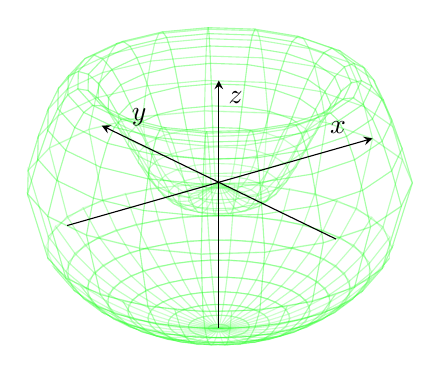
\begin{tikzpicture}
        \begin{axis}[colormap/hot2, 
            xlabel = $x$, ylabel = $y$, zlabel = $z$, 
            view = {-37.5}{30}, 
            ticks = none,
            axis lines=center, 
            axis on top,
            grid = major,]
        \addplot3 [surf,
            opacity = 0.2,           
            faceted color=green,
            white,
            z buffer=sort,
            trig format plots=rad,
            samples=20, 
            domain=0:2*pi,
            y domain=-3*pi/2:3*pi/2,
            variable=t,
            variable y=r,
            grid = major,]
            ({r*cos(t)}, {r*sin(t)}, {-sqrt((2.25*(pi)^2) - r^2) });
        \addplot3 [surf,
            opacity = 0.2,
            faceted color=green,
            white,
            z buffer=sort, 
            trig format plots=rad,
            samples=20, 
            domain=0:2*pi, 
            y domain=0:3*pi/2,
            variable=t, 
            variable y=r]
            ({r*cos(t)}, {r*sin(t)}, {-r*cos(r)});
        \end{axis}
      \end{tikzpicture}
\end{center}
Khối $\Omega_1$ được giới hạn bởi 2 mặt cong có miền lần lượt là:
\[
    (1) : \begin{cases}
        0 \leq r \leq \dfrac{3\pi}{2} \\
        0 \leq \varphi \leq 2\pi \\
        0 \leq z \leq -r\cos r 
    \end{cases}    \text{ và }
    (2) : \begin{cases}
        0 \leq r \leq \dfrac{3\pi}{2} \\
        0 \leq \varphi \leq 2\pi \\
        -\sqrt{\dfrac{9\pi^2}{4} - r^2}  \leq z \leq 0
    \end{cases}
\]
Thể tích của khối $\Omega_1$ đã cho là
\[
V = \displaystyle \int_{0}^{\dfrac{3\pi}{2}}r\mathrm{d}r\int_{0}^{2\pi}\mathrm{d} \varphi\int_{0}^{-r\cos r}\mathrm{d}z + \int_{0}^{\dfrac{3\pi}{2}}r\mathrm{d}r\int_{0}^{2\pi}\mathrm{d} \varphi\int_{-\sqrt{9\pi^2 / 4 - r^2}}^{0}\mathrm{d}z =\dfrac{9\pi^3}{2} -4\pi +  \dfrac{9\pi^4}{4} 
\]

Kết quả khi vẽ khối $\Omega_1$ trong MATLAB:
\begin{figure}[h!]
    \centering
    \includegraphics[width = 0.45\textwidth]{figure1.png}
    \caption{Khối $\Omega_1$}
\end{figure}
\newpage
\begin{comment}
CODE THAM KHẢO VẼ HÌNH LATEX 
    \begin{center}
    %x^2 + y^2 + z^2 = 1
    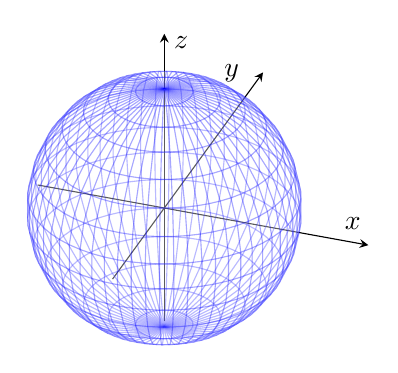
\begin{tikzpicture}
    \begin{axis}[%
        axis equal,
        width=10cm,
        height=10cm,
        axis lines = center,
        xlabel = {$x$},
        ylabel = {$y$},
        zlabel = {$z$},
        xmax=1.1,xmin=-0.5,
        ymax=1.5,ymin=-0.5,
        zmax=1.01,zmin=-0.5,
        ticks=none,
        enlargelimits=0.3,
        view/h=20,
        scale uniformly strategy=units only,
    ]
    \addplot3[%
        opacity = 0.2,
        surf,
        faceted color=blue,
    	white,
        z buffer = sort,
        samples = 31,
        variable = \u,
        variable y = \v,
        domain = 0:180,
        y domain = 0:360,
    ]
    ({cos(u)*sin(v)}, {sin(u)*sin(v)}, {cos(v)});
    \end{axis}
    \end{tikzpicture}
    \end{center}
\end{comment}
\textbf{Đoạn code mô phỏng.}
\lstinputlisting[language=Matlab]{fig1.m}
\subsection{Khối $\Omega_2$}
Vật thể $\Omega_2$ xác định bởi khối $\rho \leq 1 - \cos(\theta), \thickspace 0 \leq \theta \leq \pi$ và đường cong $\rho = 2\sin(2\theta), \thickspace \varphi = 0$ trong tọa độ cầu.
\begin{comment}
    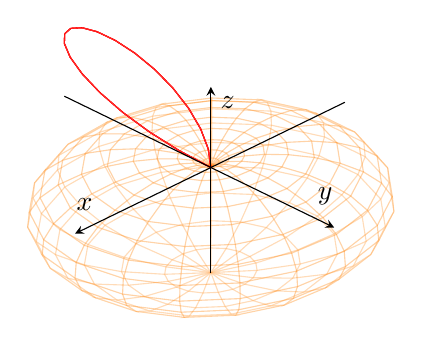
\begin{tikzpicture}
        \begin{axis}[colormap/hot2, 
            xlabel = $x$, ylabel = $y$, zlabel = $z$, 
            view = {135}{45}, 
            ticks = none, 
            axis lines=center, 
            axis on top,
            grid = major,]
        \addplot3 [surf,
            opacity = 0.2,           
            faceted color= orange,
            white,
            z buffer=sort,
            trig format plots=rad,
            samples=20, 
            domain=0:2*pi,
            y domain=0:pi,
            variable=\b,
            variable y=\a,
            grid = major,]
            ({(1- cos(a))*sin(a)*cos(b)}, {(1- cos(a))*sin(a)*sin(b)}, {(1- cos(a))*cos(a)});
        \addplot3 [surf,
            opacity = 0.2,           
            faceted color= red,
            white,
            z buffer=sort,
            trig format plots=rad,
            samples=20, 
            domain=0.5*pi:pi,
            %y domain0:pi,
            variable=\a,
            %variable y=\a,
            grid = major,]
            ({0}, {2*sin(2*a)*sin(a)}, {2*sin(2*a)*cos(a)});
        \end{axis}
      \end{tikzpicture}
\end{comment}
\begin{center}
    \includegraphics*[scale = 0.5]{2.png}
\end{center}
Khối $\Omega_2$ giới hạn bởi:
\[
    \begin{cases}
        0 \leq \theta \leq \pi \\
        0 \leq \rho \leq 1 - \cos \theta \\
        0 \leq \varphi \leq 2\pi
    \end{cases}    
\]
Thể tích khối $\Omega_2$:
\[
    V = \int_{0}^{2\pi} \int_{0}^{\pi} \int_{0}^{1-\cos \theta}\rho^2 \sin \theta \mathrm{d}\rho \,\mathrm{d} \theta \, \mathrm{d}\varphi = \frac{8\pi}{3}    
\]
\newpage
Kết quả khi vẽ khối $\Omega_2$ trong MATLAB:
\begin{figure}[h!]
    \centering
    \includegraphics[width = 0.8\textwidth]{figure3.png}
    \caption{Khối $\Omega_2$}
\end{figure}

\textbf{Đoạn code mô phỏng.}
\lstinputlisting[language=Matlab]{fig3.m}

\subsection{Khối $\Omega_3$}
Khối $\Omega_3$ giới hạn bởi hai mặt cong $x^2 + z^2 - \dfrac{y^2}{16} = 1$ và hai mặt phẳng song song, đối xứng nhau qua $Oxz$.
\begin{center}
    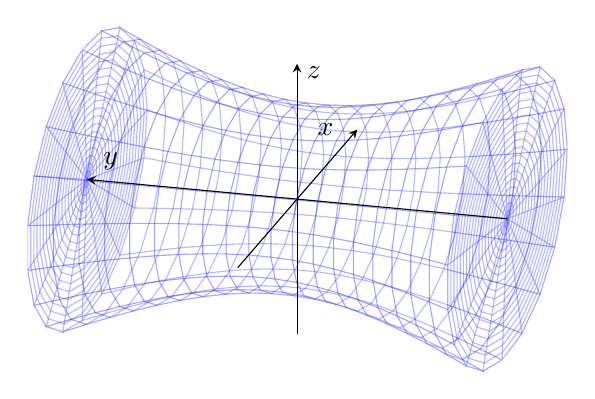
\begin{tikzpicture}
        \begin{axis}[colormap/hot2, 
            xlabel = $x$, ylabel = $y$, zlabel = $z$, 
            view = {-74.1055}{27.9581}, 
            ticks = none, 
            axis lines=center, 
            axis on top,
            grid = major,]
        \addplot3 [surf,
            opacity = 0.2,           
            faceted color=blue,
            white,
            z buffer=sort,
            trig format plots=rad,
            samples=20, 
            domain=0:2*pi,
            y domain=0:sqrt(41)/4,
            variable=t,
            variable y=r,
            grid = major,]
            ({r*cos(t)}, {5}, {r*sin(t)});
        \addplot3 [surf,
            opacity = 0.2,           
            faceted color=blue,
            white,
            z buffer=sort,
            trig format plots=rad,
            samples=20, 
            domain=0:2*pi,
            y domain=0:sqrt(41)/4,
            variable=t,
            variable y=r,
            grid = major,]
            ({r*cos(t)}, {-5}, {r*sin(t)});
        \addplot3 [surf,
            opacity = 0.2,
            faceted color=blue,
            white,
            z buffer=sort, 
            trig format plots=rad,
            samples=20, 
            domain=0:2*pi, 
            y domain=-5:5,
            variable = \t,
            variable y = \u,]
            ({sqrt(1 + (u^2)/(16))*cos(t)}, {u}, {sqrt(1 + (u^2)/(16))*sin(t)});
        \end{axis}
      \end{tikzpicture}
\end{center}
Gọi 2 mặt phẳng song song, đối xứng qua $Oxz$ là $y = \pm k,\thickspace k \in \mathbb{R}$. Đặt $x=r\cos \varphi$, $z = r\sin \varphi$. Chiếu khối $\Omega_3$ lên Oxz ta được miiền:
\[
    \begin{cases}
        0 \leq r \leq \sqrt{1 + \frac{k^2}{16}} \\
        0 \leq \varphi \leq 2\pi \\
        -k \leq y \leq k
    \end{cases}    
\]
Thể tích của khối $\Omega_3$ đã cho theo tọa độ trụ:
\[
    V_3 =  \int_{0}^{\sqrt{1 + \dfrac{y^2}{16}}}r\mathrm{d}r\int_{0}^{2\pi}\mathrm{d}\varphi\int_{-k}^{k}\mathrm{d}y = 2\pi k+ \frac{\pi k^3}{8}
\]
Kết quả khi vẽ khối $\Omega_3$ trong MATLAB:
\begin{figure}[h!]
    \centering
    \includegraphics[scale = 0.525]{figure2.png}
    \caption{Khối $\Omega_3$}
\end{figure}
\newpage
\textbf{Đoạn code mô phỏng.}
\lstinputlisting[language=Matlab]{fig2.m}
\section{Câu 2}
Chọn khối $\Omega_3$ giới hạn bởi $x^2 + z^2 - \dfrac{y^2}{16} = 1$ và hai mặt phẳng song song, đối xứng qua Oxz.

Gọi hai mặt phẳng song song, đối xứng qua Oxz là $y = \pm a$, dựa vào hình vẽ ta thấy $y$ chạy từ $-a$ tới $a$ nên ta xét đoạn $-a \leq y \leq a$.

Gọi $n$ là số mặt cắt $\Rightarrow h = \dfrac{2a}{n-1}$ $(n > 1)$ là khoảng cách giữa hai mặt cắt. Vì những mặt cắt qua một khối đều có dạng là hình tròn khi chiếu xuống mặt $Oxz$ nên ta tính diện tích từng mặt cắt bằng công thức $S = \pi R^2$, với $R^2 = 1 + \dfrac{y^2}{16}$. Vậy $S = \pi \left( 1 + \dfrac{y^2}{16} \right) = \dfrac{\pi}{16}\left( 16+ y^2 \right)$.
\begin{itemize}
    \item $y_0 = -a \Rightarrow S_0 = \dfrac{\pi}{16}\left( 16+ a^2 \right)$.
    \item $y_1 = -a + h = \dfrac{-a(n-3)}{n-1} \Rightarrow S_1 = \dfrac{\pi}{16}\left( 16+ a^2\left(\dfrac{n-3}{n-1} \right)^2\right)$.
    \item $y_2 = -a + 2h = \dfrac{-a(n-5)}{n-1} \Rightarrow S_2 = \dfrac{\pi}{16}\left( 16+ a^2\left(\dfrac{n-5}{n-1} \right)^2\right)$.
    \item $y_3 = -a + 3h = \dfrac{-a(n-7)}{n-1} \Rightarrow S_3 = \dfrac{\pi}{16}\left( 16+ a^2\left(\dfrac{n-7}{n-1} \right)^2\right)$.
    \item $\ldots$
    \item $y_k = -a + kh = \dfrac{-a(n-2k-1)}{n-1} \Rightarrow S_k = \dfrac{\pi}{16}\left( 16+ a^2\left(\dfrac{n-2k-1}{n-1} \right)^2\right)$.
\end{itemize}
Tổng của $n$ mặt cắt qua một khối.
\[
    S = S_0 + S_1 + S_2 + \ldots + S_n
\]
\[
    \Rightarrow S = \frac{\pi}{16}\left(16n + a^2 + a^2\left(\dfrac{n-3}{n-1} \right)^2 + a^2\left(\dfrac{n-5}{n-1} \right)^2 + \ldots + a^2\left(\dfrac{n-2k-1}{n-1} \right)^2 \right)    
\]
\[
    \Rightarrow S = n\pi +  \dfrac{\pi a^2}{8}\left(1 + \left(\dfrac{n-3}{n-1} \right)^2 + \left(\dfrac{n-5}{n-1} \right)^2 +\ldots+ \left(\dfrac{n-2k-1}{n-1} \right)^2\right)    
\]
Trong đó
\begin{itemize}
    \item Nếu $n$ lẻ thì ta tính tới $n - 2k - 1 = 0$.
    \item Nếu $n$ chẵn thì ta tính tới $n - 2k - 1 = 1$. 
\end{itemize}
Ta chọn hai mặt phẳng song song, đối xứng nhau qua $Oxz$ là $y = 10$ và $y = -10$ với $n = 101$ mặt cắt. Áp dụng theo công thức trên ta được diện tích $101$ mặt cắt là:
\[
    S = n\pi +  \dfrac{\pi a^2}{8}\left(1 + \left(\dfrac{n-3}{n-1} \right)^2 + \left(\dfrac{n-5}{n-1} \right)^2 +\ldots+ \left(\dfrac{n-101}{n-1} \right)^2\right)    
\]
\[
   \Rightarrow S = 101\pi + \dfrac{\pi 10^2}{8}\left( 1 + \left(\frac{101-3}{101-3}\right)^2 + \left(\frac{101-5}{101-1}\right)^2 + \ldots + \left(\frac{101-101}{101-1}\right)^2  \right)    
\]
\[
    \Rightarrow S = 101\pi + \dfrac{1717\pi}{8} \approx 991.5652   
\]
\textbf{Đoạn code mô phỏng.}
\lstinputlisting[language=Matlab]{code.m}
Kết quả chạy trên MATLAB: 
\begin{center}
    \includegraphics[scale = 0.8]{image.png}
\end{center}
\section{Kết luận}
Thông qua quá trình nghiên cứu, tìm tòi và học hỏi dưới sự dẫn dắt nhiệt tình của cô Trần Thị Ngọc Huyền, nhóm 2 chúng em đã hoàn thành được đề tài nghiên cứu đồng thời mở rộng thêm được nguồn kiến thức trên nhiều phương diện khác nhau.

Về phần môn học Giải tích 2, sau khi giải quyết được các bài tập mà cô đưa ra, chúng em nhận thấy rằng mình hiểu hơn về môn học cũng như có thêm môi trường để vận dụng những kiến thức mà chúng em nhận được trong quá trình học tập từ lối tư duy đưa ra hưởng giải bài, tới cách áp dụng công thức và trình bày bài giải một cách rõ ràng, cụ thể. Đây có thể coi như một cơ hội để chúng em ôn lại phần kiến thức đã học và giúp chúng em ghi nhớ kỹ hơn thông qua việc tự nghiên cứu chuyên sâu vấn đề.

Về phần phần mềm MATLAB, chúng em đã tiến hành tìm hiểu cũng như tiếp cận đến những lệnh code từ cơ bản đến nâng cao để phục vụ quá trình thực hiện đề tài. Từ đó, giúp chúng em phát triển thêm kỹ năng lập trình, tiếp cận công nghệ tiên tiến và nâng cao sự hiểu biết của bản thân. 

Về phần báo cáo, chúng em thống nhất việc trình bày bài báo cáo này bằng \LaTeX, để đem lại sự chuyên nghiệp cũng như tăng độ thẩm mỹ. Đây là một phần mềm khá phổ biến và được đề cao trong giới nghiên cứu học thuật, là một trong những lựa chọn hàng đầu của các nhà nghiên cứu khoa học khi trình bày các bài báo khoa học từ cấp đơn vị đến quốc tế.
\newpage
\section*{Tài liệu tham khảo}
\begin{itemize}
    \item[1] Holly Moore, \textit{MATLAB for Engineers: (5th Edition)}, Pearson, 2017.
    \item[2] Nguyễn Đình Huy (Chủ biên), Lê Xuân Đại, Ngô Thu Lương, Nguyễn Bá Thi, Trần Ngọc Diễm, Đậu Thế Phiệt, \textit{Giáo trình Giải tích 2}, NXBDHQG, 2009.
    \item[3] James Stewart, \textit{Calculus: Early Transcendentals (6th Edition)}, Cengage Learning, 2007.
\end{itemize}
\end{document}